\documentclass{standalone}
\usepackage{tikz}
\begin{document}
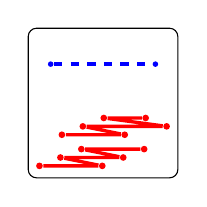
\begin{tikzpicture}[scale=1.9]
  % draw rounded cell boxes
  \draw[rounded corners=3pt] (0,0) rectangle (1,1);
  % draw black chords for chord_row_cells
  \node[circle, fill=red, inner sep=0.03cm] (obs4363485504_pt0) at (0.075,0.08) {};
  \node[circle, fill=red, inner sep=0.03cm] (obs4363485504_pt1) at (0.21499999999999997,0.136) {};
  \node[circle, fill=red, inner sep=0.03cm] (obs4363485504_pt2) at (0.3549999999999999,0.192) {};
  \node[circle, fill=red, inner sep=0.03cm] (obs4363485504_pt3) at (0.49499999999999994,0.08) {};
  \node[circle, fill=red, inner sep=0.03cm] (obs4363485504_pt4) at (0.635,0.136) {};
  \node[circle, fill=red, inner sep=0.03cm] (obs4363485504_pt5) at (0.775,0.192) {};
  \draw[red, line width=1.2pt] (obs4363485504_pt0) -- (obs4363485504_pt3) -- (obs4363485504_pt1) -- (obs4363485504_pt4) -- (obs4363485504_pt2) -- (obs4363485504_pt5);
  \node[circle, fill=red, inner sep=0.03cm] (obs4363485360_pt0) at (0.22499999999999998,0.28800000000000003) {};
  \node[circle, fill=red, inner sep=0.03cm] (obs4363485360_pt1) at (0.365,0.34400000000000003) {};
  \node[circle, fill=red, inner sep=0.03cm] (obs4363485360_pt2) at (0.5049999999999999,0.4) {};
  \node[circle, fill=red, inner sep=0.03cm] (obs4363485360_pt3) at (0.6449999999999999,0.28800000000000003) {};
  \node[circle, fill=red, inner sep=0.03cm] (obs4363485360_pt4) at (0.7849999999999999,0.4) {};
  \node[circle, fill=red, inner sep=0.03cm] (obs4363485360_pt5) at (0.9249999999999999,0.34400000000000003) {};
  \draw[red, line width=1.2pt] (obs4363485360_pt0) -- (obs4363485360_pt3) -- (obs4363485360_pt1) -- (obs4363485360_pt5) -- (obs4363485360_pt2) -- (obs4363485360_pt4);
  \node[circle, fill=blue, inner sep=0.025cm] (req4363337504_pt0) at (0.15,0.76) {};
  \node[circle, fill=blue, inner sep=0.025cm] (req4363337504_pt1) at (0.85,0.76) {};
  \draw[blue, dashed, line width=1.2pt] (req4363337504_pt0) -- (req4363337504_pt1);
\end{tikzpicture}
\end{document}